\documentclass[a4paper,11pt]{article}

\usepackage{graphicx}
\usepackage{url}

\setlength{\textheight}{9.50in}
\setlength{\textwidth}{6.75in}
\setlength{\topmargin}{-0.40in}
\setlength{\oddsidemargin}{-0.125in}
\setlength{\evensidemargin}{-0.375in}
\setlength{\columnsep}{2pc}
\setlength{\headheight}{0.200in}
\setlength{\headsep}{0.4in}
\setlength{\footskip}{0.450in}
\setlength{\parindent}{1em}
\flushbottom

\begin{document}

\noindent {\large Rijkswaterstaat and Esri Nederland}

\vspace{0.5em}

\noindent {\bf\LARGE Social Media as (safe) enabler of the participation society}

\vspace{2em}

\noindent Wouter Meulemans$^1$, Robert Boensma$^2$, Ana-Maria Oprescu$^3$, Hannes M\"uhleisen$^4$, Marco Aiello$^5$, Kaifeng Yang $^6$, Ugo Vespier $^6$

\vspace{1em}

\noindent Marcel de Rink$^7$

\vspace{1em}

\noindent $^1$ \emph{Technische Universiteit Eindhoven, The Netherlands}\\
\noindent $^2$ \emph{Universiteit Twente, The Netherlands}\\
\noindent $^3$ \emph{University of Amsterdam, The Netherlands}\\
\noindent $^4$ \emph{Centrum Wiskunde \& Informatica, Amsterdam, The Netherlands}\\
\noindent $^5$ \emph{LIACS Leiden University, The Netherlands}\\
\noindent $^6$ \emph{Rijksuniversiteit Groningen, The Netherlands}\\
\noindent $^7$ \emph{ESRI, The Netherlands}

\section{Abstract}

The increasingly ubiquitous nature of the digital society opens 
new avenues for social innovation. A difficult challenge in this context
is to correctly identify new types of trade-offs, as well as envision 
promising strategies. As a concrete case study, we analyze the direct society participation
in the complete process of bike lane maintenance. In this report, we identify 
key aspects to consider when designing such a framework, as well as describe
our approach to obtaining a trade-off between bike lane safety and 
bike lane information accuracy, by leveraging off-the-shelf technology like smartphones.
Our approach shows promising initial results and underlines the areas of interest for a future 
working group.
 

\section{Company profile}

\subsection*{Esri Nederland}

Esri offers customers technology to enables organizations to create responsible and sustainable solutions to problems at local and global scales. Esri tries to make our customers successful.
Esri (as global company) is driven by innovation.
Esri's annual revenues were indicated to be \$1.2 billion (see Wikipedia).
Esri spent more than 20\% of the turnover on renewal, innovation and R\&D to embed new technology in the software to offer customers the latest technology.
At Esri, we believe that geography is at the heart of a more resilient and sustainable future.

\subsection*{Rijkswaterstaat}

Rijkswaterstaat is part of the Dutch Ministry of Infrastructure and the Environment and responsible for the design, construction, management and maintenance of the main infrastructure facilities in the Netherlands. This includes the main road network, the main waterway network and the main water systems.
A relative new area of interest for Rijkswaterstaat is social innovation and, a.o. we're looking into the possibilities of citizen participation and crowd sourcing to improve our work processes.

\section{Problem description}

The Dutch government is positioning the participation society. Social Media is an important way to interact with citizens, companies and government. Safe use of social media is also important. At the moment, the Government launches a campaign about safe use of social media eg ``don't use it while driving''.
The results of the Workshop 'ICT with Industry' will be used for the project `improving safety on bike lines'. This is a pilot project for Rijkswaterstaat on co-creation in which Rijkswaterstaat, Esri Nederland (and Lemon Innovation), with help of the Dutch cyclists association (fietsersbond), try to improve safety on our bike lanes. Around 80\% of the necessary information (on where unofficial bike lanes are located, condition of the lanes and safety issues) is available based on existing databases, maps and data mining. The gaps have to be filled in by the cyclists themselves. Cyclists are willing to provide this information, at least, if it takes little effort; e.g. use twitter while driving. This conflicts with the Dutch policy of `safe use of social media'.
Our problem is `how can citizens (e.g. cyclist) provide information about the infrastructure facilitates in the Netherlands without significant extra effort and without endangering their safety'.
Conditions are that citizens (or the government) should not have to invest in expensive sensors (i.e. common devices like smart phones should be used) and that not a lot of effort is involved (e.g. stop cycling, measure the width of the road, send a message or fill in a form on a website).

\section{Problem analysis}

Based on the problem description, we decided to focus on determining road quality. The system should have a low threshold of participation, for both the cyclist and RWS.
Thus we decided that as many steps as realistically possible should be automated.

\subsection{Nontechnical considerations}

Before we can investigate possible designs and techniques, we first answer three questions:
\begin{enumerate}\setlength{\itemsep}{-3pt}
\item What determines road quality?
\item What are possible stakeholders for the system?
\item What incentives can we provide for cyclists to participate?
\end{enumerate}

\subsubsection{Road quality}

We distinguish a number of properties that together contribute to road quality in a very broad sense. The importance of some properties depends on the type of cyclist (e.g. racing, recreational, commuter).
\begin{itemize}\setlength{\itemsep}{-3pt}
\item \textbf{Damage and obstacles}: damaged roads and obstacles detract heavily from road quality. They may cause accidents and contribute to an increased wear of bikes.
\item \textbf{Road-surface smoothness}: the smoothness of the road surface also affects the quality. Asphalt tends to be more comfortable to ride on than cobble stones. However, there is a caveat in trying to determine road quality here: we do not want to simply conclude that all cobble-stone roads must be replaced with asphalt.
\item \textbf{Weather}: weather may affect road quality in a variety of ways. For example, a road that is prone to flooding with heavy rain may need to be avoided in some cases. Icy roads increase the chance of slipping and falling: under such conditions, roads next to rivers or canals are more dangerous than they would be under normal circumstances. These weather effects may also cause for seasonal changes in road quality.
\item \textbf{Traffic}: congested areas and busy bike lanes lead to increased travel times and increased chances of accidents.
\item \textbf{Air pollution}: air pollution is detrimental to the quality of a road. Factories or motorized traffic may cause local pollution Thus, for example, bike lanes in industrial areas or near often-congested roads may be considered of lower quality.
\item \textbf{Lighting}: good lighting contributes to safety. Poor lighting may cause damage or obstacles to be barely visible, leading to an increased chance of accidents. However, good lighting also contributes to a sense of social safety.
\item \textbf{Signalling}: good signaling along the bike lanes is beneficial to route quality. This may have little value for a commuter who knows his route. However, for a recreational cyclist, signaling may be of great value.
\end{itemize}

\subsubsection{Stakeholders}

Let us know turn to analyzing stakeholders of a system that determines road quality.

\paragraph{Road authorities.}
For RWS as well as local governments, knowledge on road quality may be valuable in determining where unsafe or congested areas are. Such knowledge enables efficient and effective actions to be taken to improve upon hazardous situations, thereby improving road quality.

\paragraph{Bike providers.}
Bike-rental companies (e.g. OV-fiets) may benefit from improved road quality. Better roads lead to less wear and tear of bikes, thus reducing maintenance costs. Here, we see also a potential for collaboration: rental bikes may be equipped with simple devices to make anonymous recordings.

\paragraph{Supporting cyclists.}
A system with information on road quality has the potential to be used by a number of other applications. For example, tourist offices can use road quality to suggest pleasant routes for a recreational cyclist. Other examples include ``ANWB Fietsen'', ``Fiets!'', ``Natuurmonumenten'' and the application developed by the fietsersbond and Eneco.

\subsubsection{Incentives for participation}

The goal of the system is to gather information on road quality. However, to be low-cost, we need participation to be voluntary and have a low threshold (e.g. little to no monetary investment). Therefore, we see a necessity to use an app installed on the cyclist's smartphone (also see Section \ref{ssec:datasource}). This app may provide a number of services in return. For example, the information on road quality allows for better route suggestions and planning. Also, the app may keep track of interesting statistics (velocity, distance traveled, calories burned, etc.). Finally, the information may allow road authorities to improve upon road quality and safety.
We may also consider the amount of (time) investment we expect of a cyclist. For hazardous situations, it would be great if the cyclist could get off his or her bike and take a photo of the situation. Also, the information quality that a cyclist can provide may be drastically increased by allowing for a cyclist to evaluate his route and automatically collected data.
However, we must estimate if this benefits appeal to a cyclist and whether a cyclist is willing to make these investments. To this end we distinguish three categories of cycling purposes: racing, recreational and commuting. For each, we briefly consider these four potential benefits and two potential investments. The results are summarized in Table \ref{tab:incentives}.

\begin{table}[b]
\centering
\begin{tabular}{l | l l l}
 & \emph{Racing} & \emph{Recreational} & \emph{Commuting}\\
\hline
\emph{Road quality} & High & Medium & Low \\
\emph{Statistics} & High & Medium & Low \\
\emph{Route suggestions} & High & High & Low \\
\emph{Road improvement} & Medium & Low & High \\
\hline
\emph{Evaluation} & High & Medium & Low \\
\emph{Make photo} & Medium & High & Low
\end{tabular}
\caption{Summary of estimated cyclist interest in benefits and willingness to invest time.}
\label{tab:incentives}
\end{table}

\paragraph{Racing.}
When a cyclist is racing, he benefits greatly from road quality. We also consider it likely that he is interested in statistics as well as route suggestions: suggestions based on road quality may avoid unpleasant surprises such as damaged roads. He is also invested in road improvement, but typically has the option of taking a different route to avoid problematic parts. We also expect racing cyclists to be willing to make some time investment in providing evaluation afterwards due to their interest in road quality. Stopping to take a photo is likely somewhat more problematic, as this requires a break from the racing schedule.

\paragraph{Recreational.}
A recreational cyclist has some interest in road quality and statistics. However, road quality (in terms of damage or surface smoothness) may not be top priority: cycling speed is typically lower and thus such issues are less problematic. The investment in road improvement is considerably lower, as recreational cyclists are likely to ride different routes on each trip. Postevaluation is less likely to come from a recreational cyclist. However, we expect such cyclists to be more than willing to stop and make a photo of a problematic situation.

\paragraph{Commuting.}
We expect that commuters are hard to reach: they have some interested in road quality and a high interest in road improvement as they travel the same or similar routes on a daily basis. However, statistics and route suggestions likely have a low appeal. Also, a commuter is unlikely to be willing to invest time into postevaluation or making photos.
However, we recognize that there might be a possible subcategory of commuters: parents who bring their children to school. While their interest in statistics and route suggestions are still low, we expect an increased interested in road quality. Also, we expect a high chance that parents are willing to perform some postevaluation or make photos after the children have been brought to school.

\subsubsection{Other considerations}

There may be a number of other considerations for the problem at hand. If a system gathers GPS data from cyclists, privacy is an important consideration. By looking at daily patterns, we may be able to establish where a cyclist works and lives, even if no user identification is stored. This is likely to narrow down the potential identity of a cyclist to one or a few citizens. Such privacy issues must be considered before a public system is deployed. However, we consider it to be out-of-scope for this workshop.

\subsection{Technical considerations}

Now that we have considered nontechnical aspects of the system, we turn our attention to the technical aspects. We consider three questions:
\begin{enumerate}\setlength{\itemsep}{-3pt}
\item What data source do we wish to use?
\item What aspects of road quality can we derive from the data?
\item Can we devise a high-level architecture for the system?
\end{enumerate}

\subsubsection{Data source}
\label{ssec:datasource}

We considered three sources of information for road quality: explicit evaluation, social media and sensor data. Below, we briefly discuss each.

\paragraph{Evaluation.}
With explicit evaluation, the system would require users to evaluate their routes and use a system where they can manually indicate problems or hazardous situations. However, this requires a high time investment of the cyclists. A system of the fietsersbond is already available that operates in this setup (\url{http://meldpunt.fietsersbond.nl/}). While this yields high-quality data, the time investment likely prohibits large-scale participation. This causes the data to only cover the most frequently traveled routes. Moreover, the absence of data may indicate two different things: the road quality is high or none took the effort of reporting problems.

\paragraph{Social media.}
With the ever-increasing participation of citizens in social media such as Facebook or Twitter, researchers and practitioners are now turning to sentiment mining for solutions to a wide array of problems. That is, text-recognition methods are used to automatically extract the opinions or sentiments of people in social media regarding certain topics. However, we expect such an approach to work poorly for road quality for a number of reasons. First, the data coverage is likely to be very low: not many people make announcements on damaged roads. Second, even if a complaint is made, it is likely hard to correlate this to an actual location: road names are not unique and possible GPS locations may correspond to a different location that the source of the complaint. Third, encouraging cyclists to use social media on bike lane problems is likely to lead to an increase of smartphone use in traffic: this is the complete opposite of the government's  ``safe use of social media'' policy.

\paragraph{Sensor data.}
Many people nowadays carry smartphones with them wherever they go. A smartphone has a wide array of sensors available that we might exploit to collect data about road quality. This needs little user investment: simply download the application and turn it on before starting a cycling trip. The device then automatically records data, which can be used for postevaluation or sent to a central system for automatic analysis. This leads to the required low investment for participants. Thus, we focus on sensor data in the remainder.

\subsubsection{Aspects of road quality}

We now investigate which aspects of road quality (see Section 4.1.1) we may determine from sensor data. A modern smartphone has a wide array of sensors, typically including the following:
\begin{itemize}\setlength{\itemsep}{-3pt}
\item \textbf{GPS}: A GPS (Global Position System) sensor allows us to record the location, speed and direction of a cyclist. This is essential in correlating measurements of other sensors to locations of problematic situations.
\item \textbf{Accelerometer and gyroscope}: These sensors allow us to measure the movement of the device. From this, we may be able to determine road damage and smoothness. A more detailed analysis and experiments for the accelerometer is provided in Section 5.
\item \textbf{Magnetometer}: A magnetometer measures changes in magnetic fields. These may be caused by passing cars and thus this sensor may allow for an estimation of traffic density.
\item \textbf{Microphone}: By recording sound levels, we may also derive traffic density.
\item \textbf{Camera}: The camera of a device can be used to make photos of a hazardous situation, to augment data with a visual representation of a problem. It may also be used to estimate the lighting conditions of the road.
\end{itemize}
However, all these sensors dramatically increase the power consumption of the device. Therefore, it may be required for cyclists to obtain a method of charging their phone (e.g. with a dynamo) while cycling. As mentioned earlier, there are also important privacy issues in recording data from some sensors, in particular the GPS sensor, microphone and camera.

\subsubsection{High-level architecture}

A potential high-level architecture of the system is given in Figure \ref{fig:architecture}. We consider three main components: the cyclist's smartphone, his base station, and the back end with a possible RWS server and other services.

\paragraph{Smartphone.}
The smartphone of the cyclist requires an application to be installed that facilitates the collection of sensor data. The smartphone may also use the gathered road-quality information in the form of other applications, such as a route planning or a statistics application (``BikeKeeper'').

\paragraph{Base station.}
If the cyclist is willing to invest time in evaluating estimates derived from sensor data or to manually provide additional information, this should be used: such derived or manual data tends to be of high quality. For this, an application on a ``base station'' (home pc, laptop, or possibly also the smartphone) can be used. This setup also allows for processing sensor data locally, sparing resources of servers as well as providing opportunities to deal with potential privacy issues.

\paragraph{Back end.}
In the back end, we consider the servers and applications that use the road-quality information or provide information for the cyclist. Its main component is the RWS server that is responsible for storing and analyzing the (sensor) data to derive road quality. For this, it may use additional information from possible affiliates such as the fietsersbond. It also proves this data for affiliates to be used in supporting services for the cyclist.

\begin{figure}
\centering
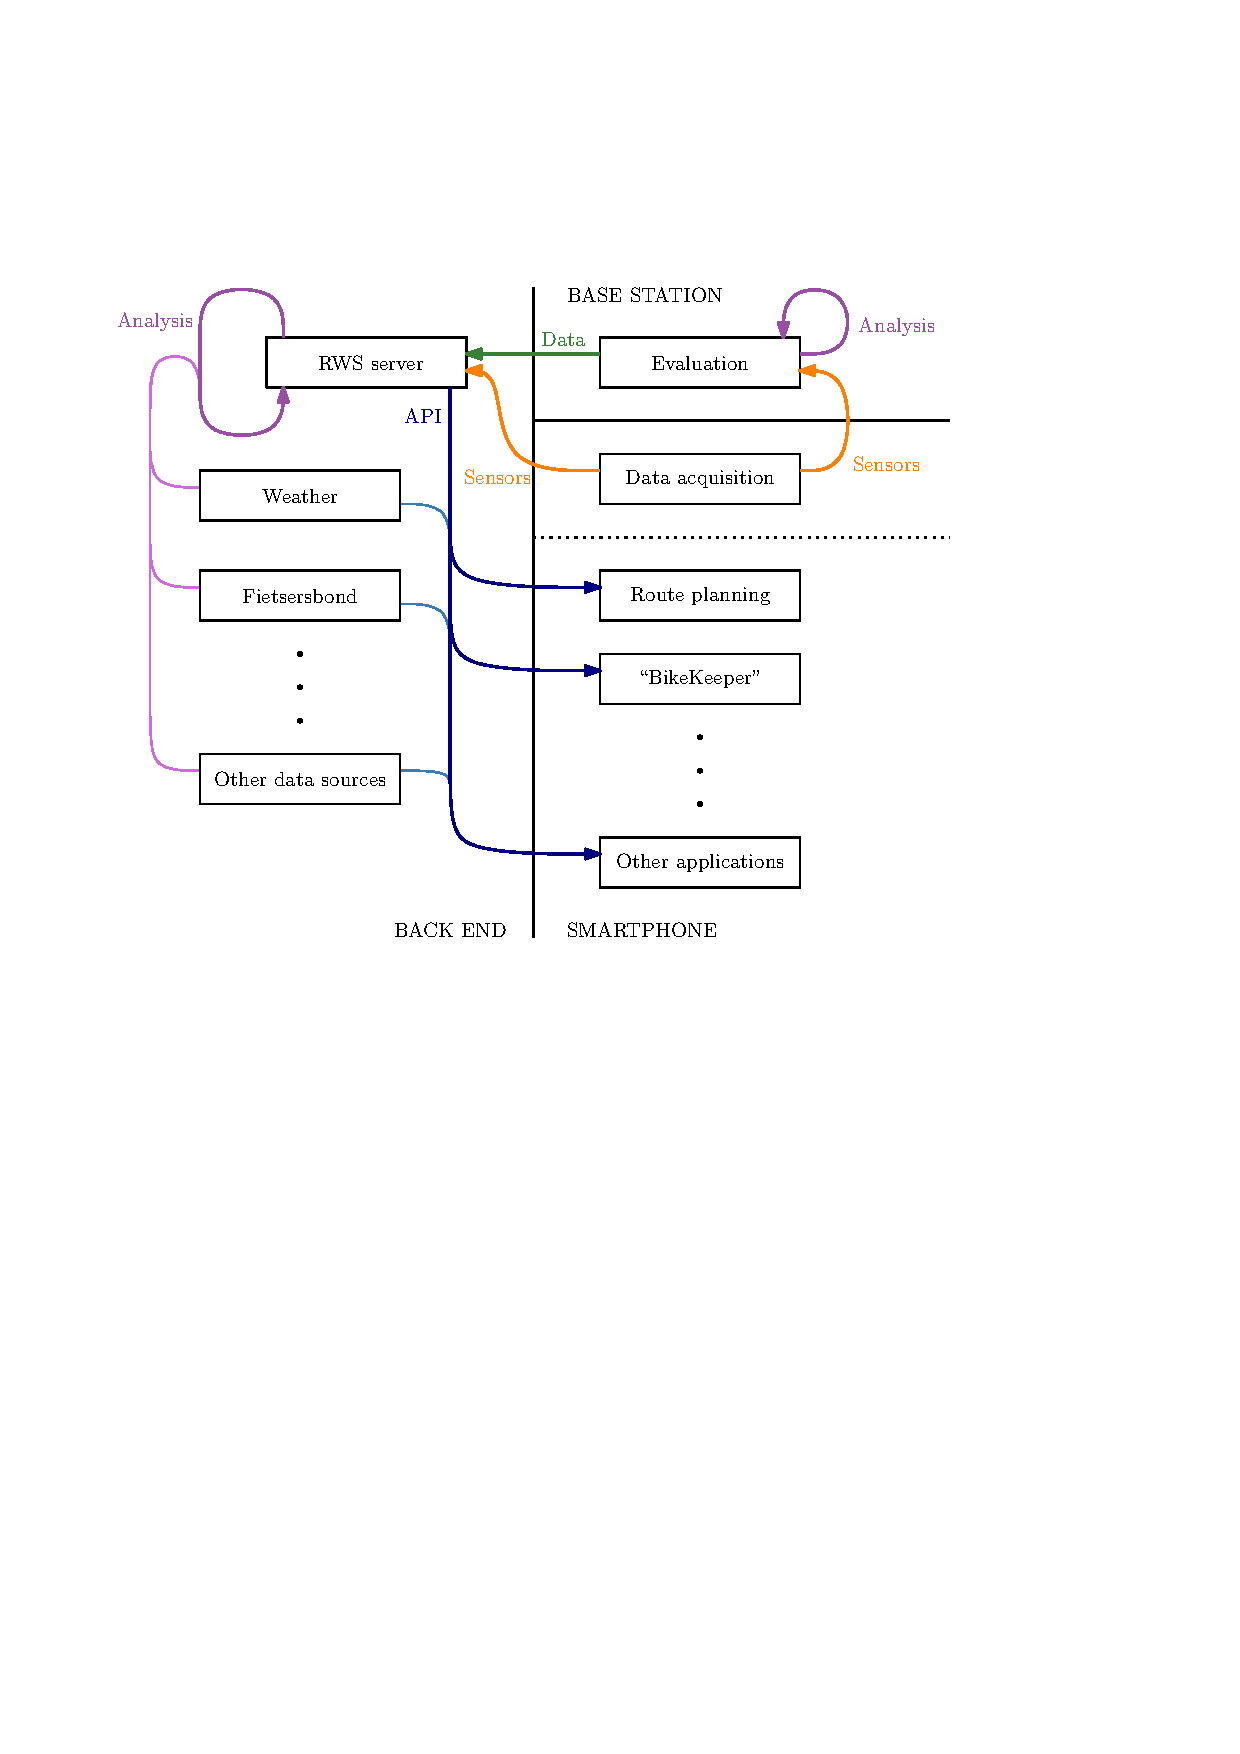
\includegraphics{figures/systemoverview}
\caption{A high-level architecture of the system. On the right: the cyclist's devices, a smartphone and a base station. Orange arrows indicate flow of sensor data. A green arrow represents evaluated data. On the left: the system back end, the RWS server and other applications and services of stakeholders. This information can be used for analysis (purple arrows) as well as combined with the obtained road-quality information to provide services to the cyclist (blue arrows).}
\label{fig:architecture}
\end{figure}

\section{Data acquisition and analysis}

An initial observation with regards to data collection was the wealth of sensors that are contain in modern ``smart'' phones. In addition, there are various applications that can record measurements from these sensors. For the initial experiment, we focused on the acceleration sensor under the assumption that bad road quality would result in additional acceleration of the rider and thus the phone. We used the free ``SensorLog'' application for Apple iOS\footnote{\url{https://itunes.apple.com/us/app/sensorlog/id388014573}} for the following experiments. Conveniently, the results are stored as CSV files, which made it easy to transfer the measurements to the R environment\footnote{\url{http://www.r-project.org}} for subsequent analysis.

\subsection{Initial Exploratory Experiment}

\begin{figure}
\centering
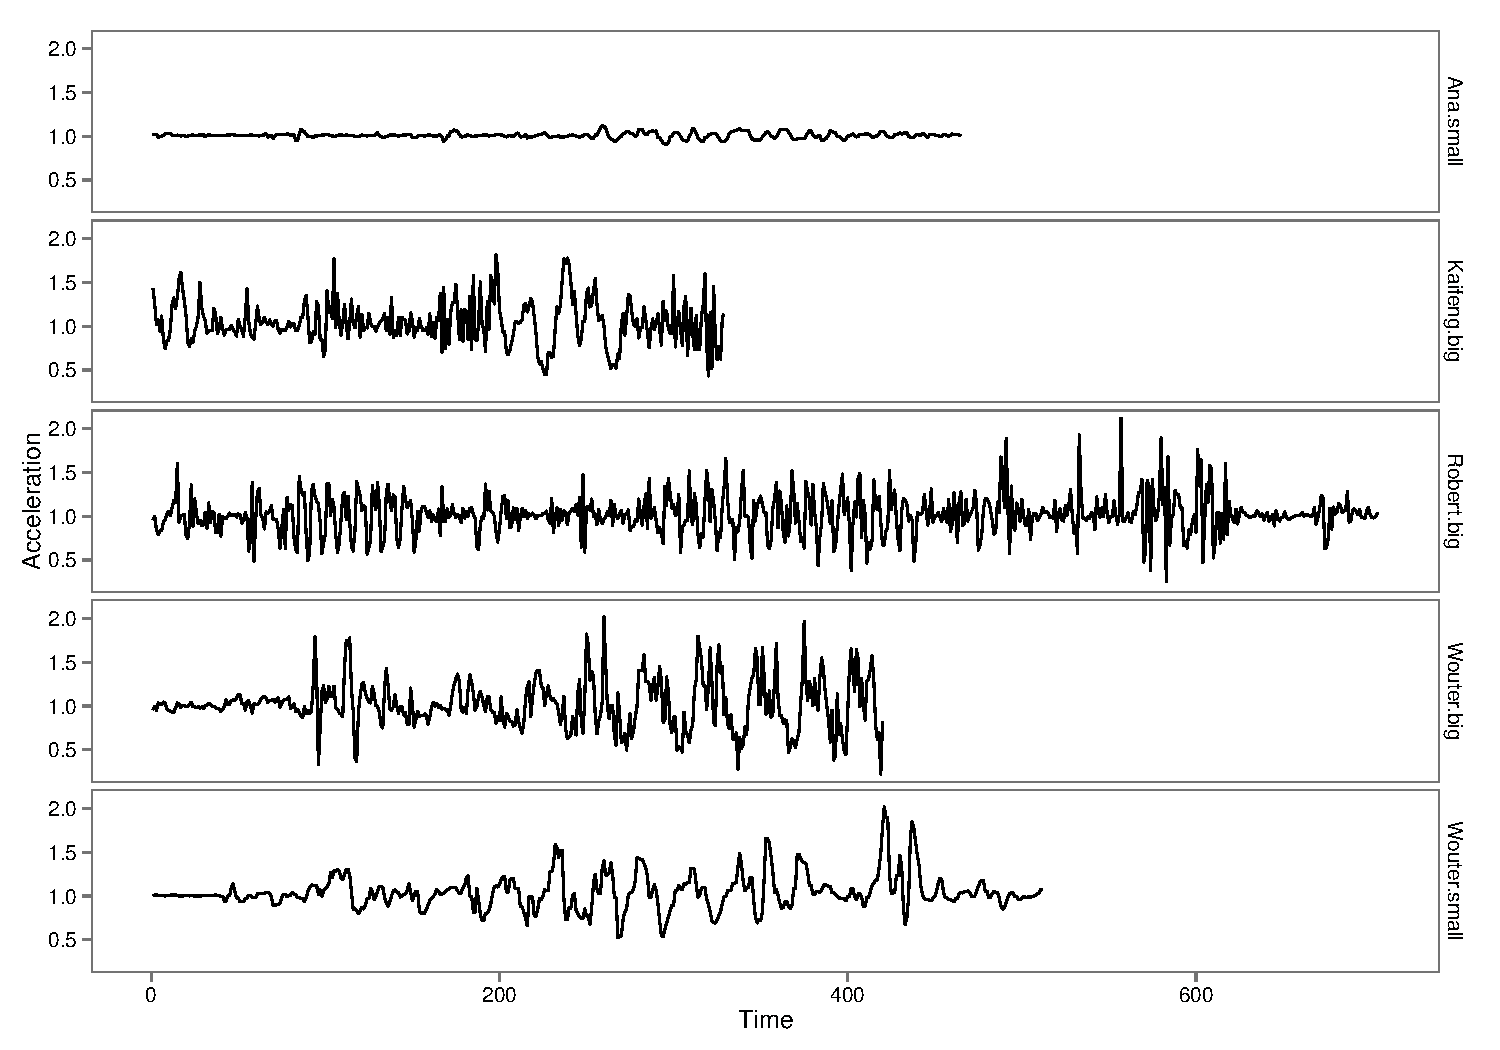
\includegraphics[width=13cm]{figures/accelerationplot}
\caption{Baseline acceleration plot}
\label{fig:accplot}
\end{figure}


In an initial experiment, we have used a number of volunteers and two different bikes on a short (~100m) piece of bike road in Leiden. On the end of the selected stretch of road, there was a significant pothole, which we encouraged the volunteers to hit. For each run, we placed the phone with SensorLog running on the person riding the bike. In total, we collected ~2,500 measurements of acceleration over five different runs. Since the acceleration data is collected in three different spatial axes $x$, $y$ and $z$, we used the Euclidean norm $||a|| = \sqrt{a_x^2+a_y^2+a_z^2}$ to calculate the length of the acceleration vector as a combined metric. The results from this initial experiemnts is plotted in Figure~\ref{fig:accplot}. We can see how the measured acceleration varies greatly between runs over the identical road surface. Also, as can be seen from the comparision of the same person (``Wouter'') between two rides on different bikes (``big'' and ``small''), there are significant deviations. Hence, the signal-to-noise ratio of these measurements was deemed to be too great for useful analysis. There was also no visible sign of the deliberatly hit pothole at the end of the track. Since we did not control for the location of the phone on the person riding the bike (sometimes it was placed in a pants pocket, sometimes in a coat pocket etc.) and observed that the individual riding style influenced the measured acceleration, we found it neccessary to further control the involved parameters.


\begin{figure}
\centering
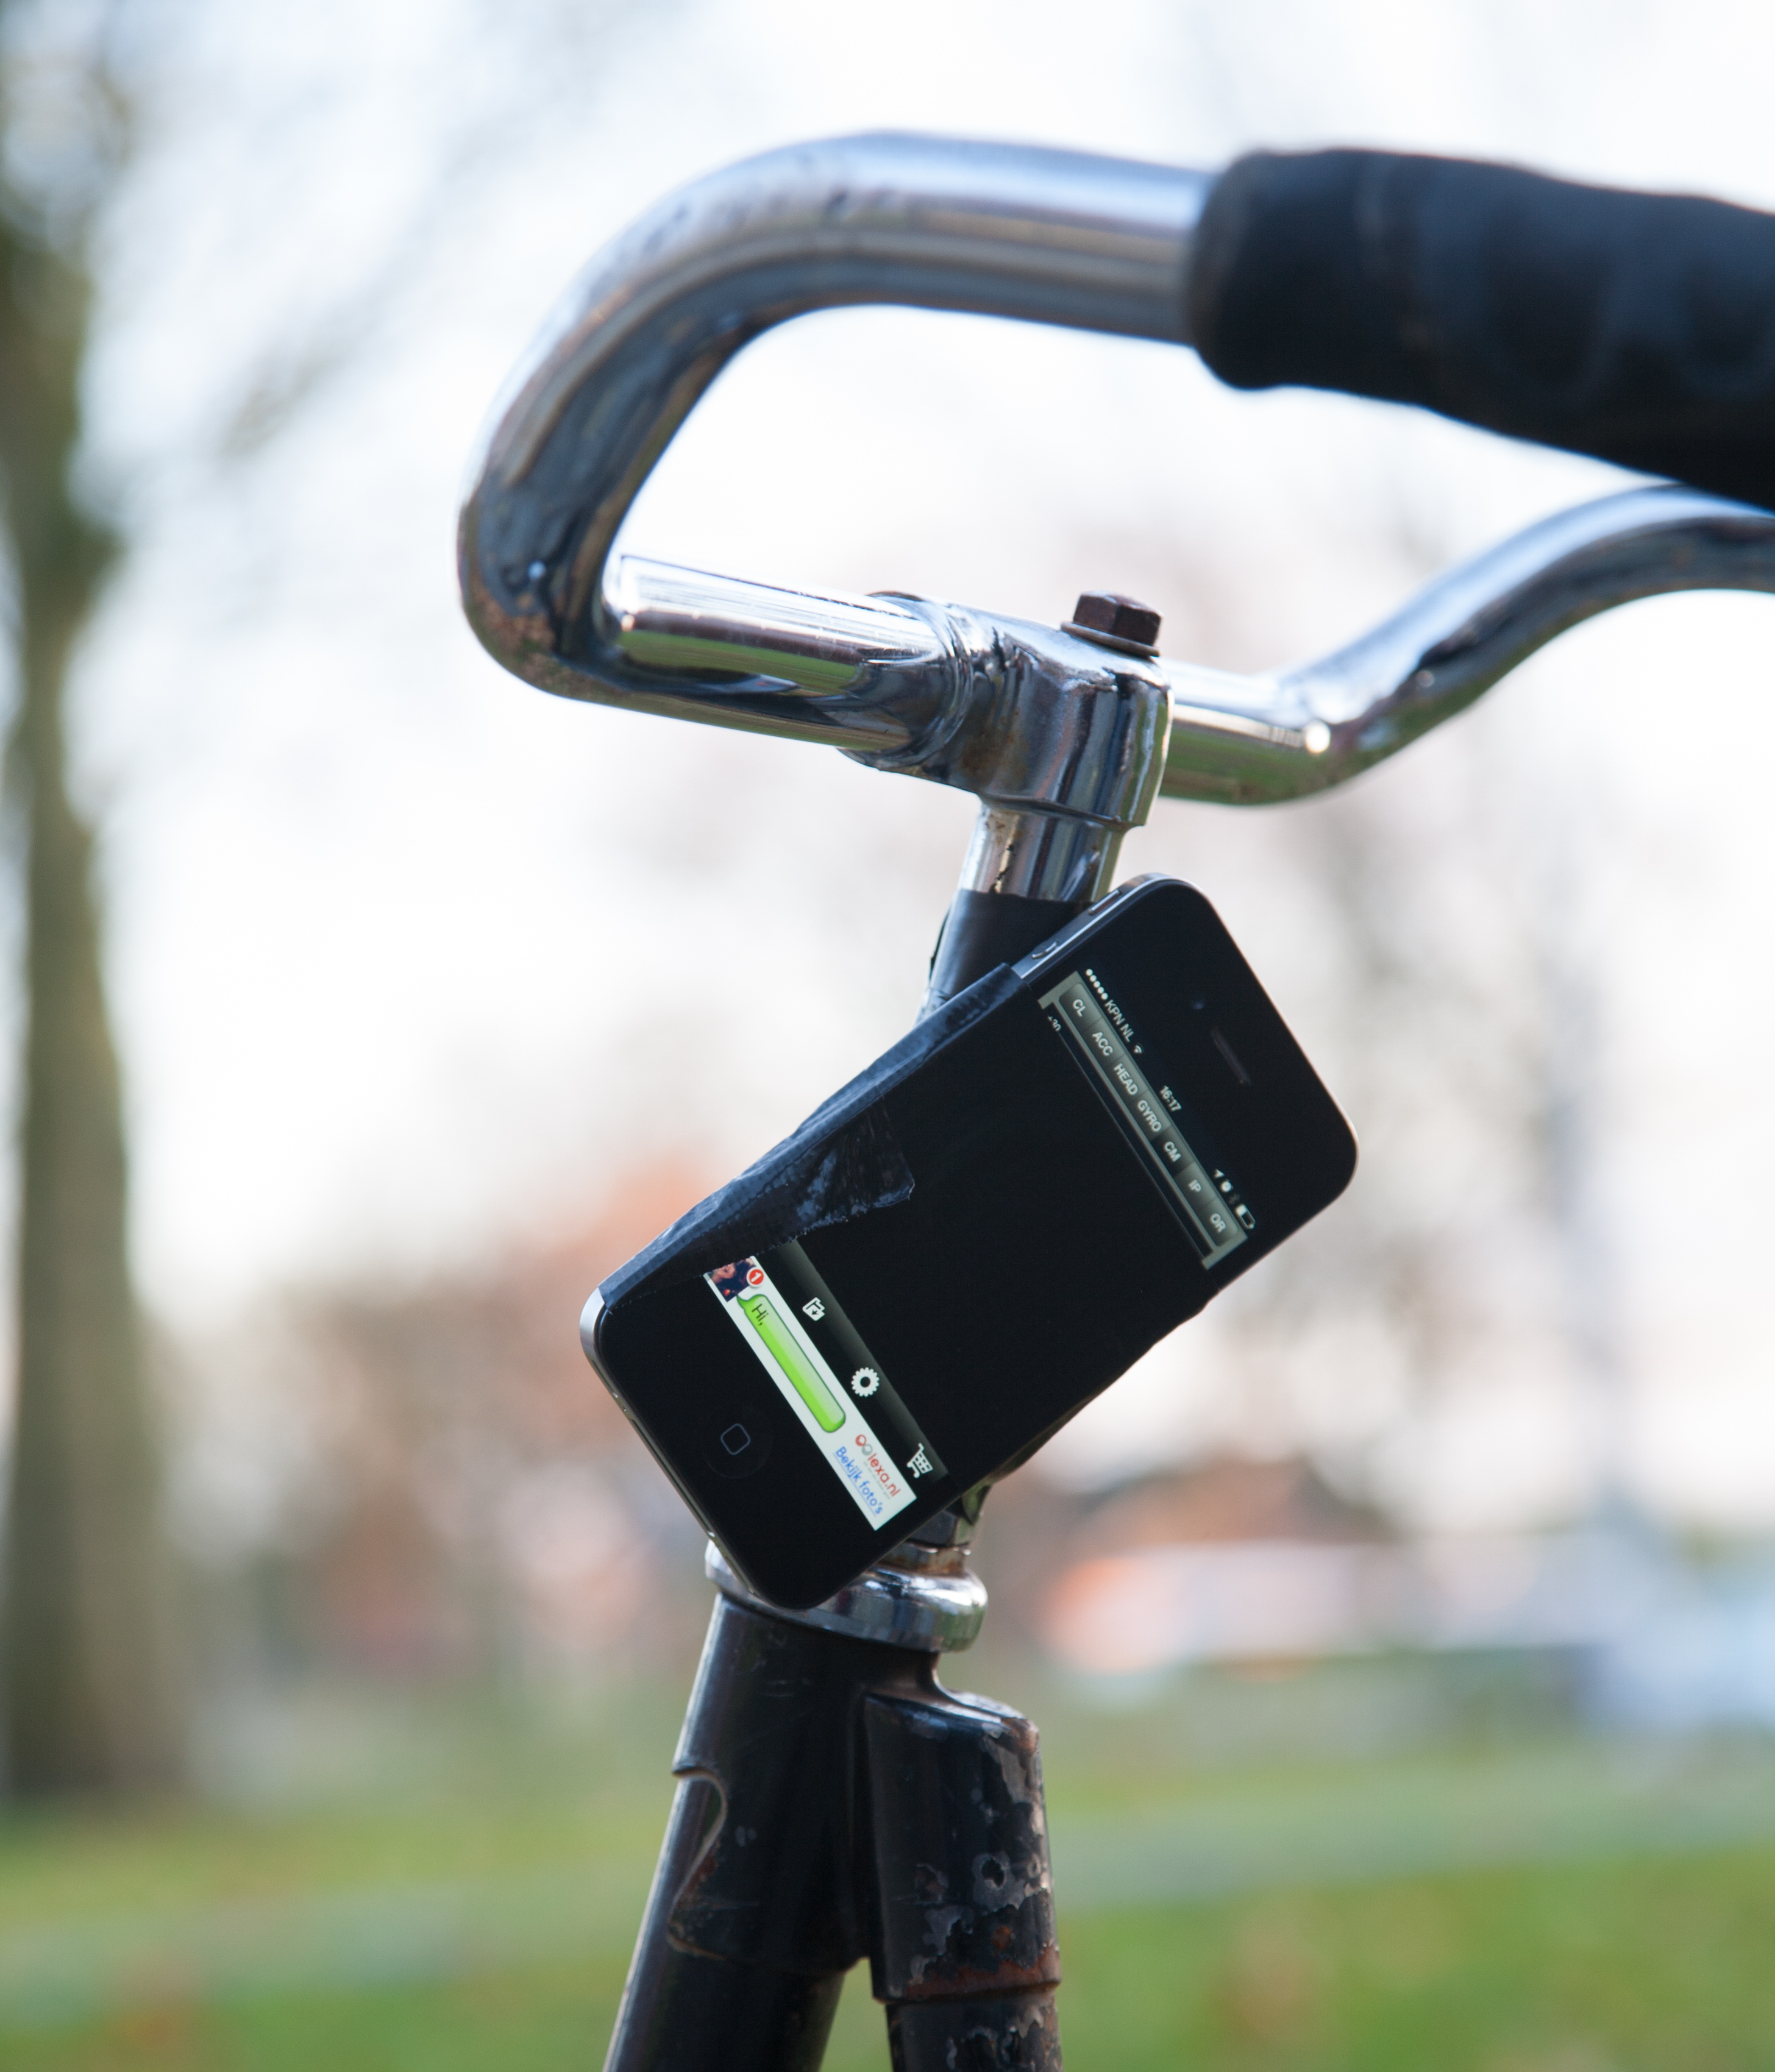
\includegraphics[width=8cm]{figures/bikec}
\caption{Experimental phone-bike attachment method}
\label{fig:exsetup}
\end{figure}


\subsection{Controlled Experiment}

\begin{figure}
\centering
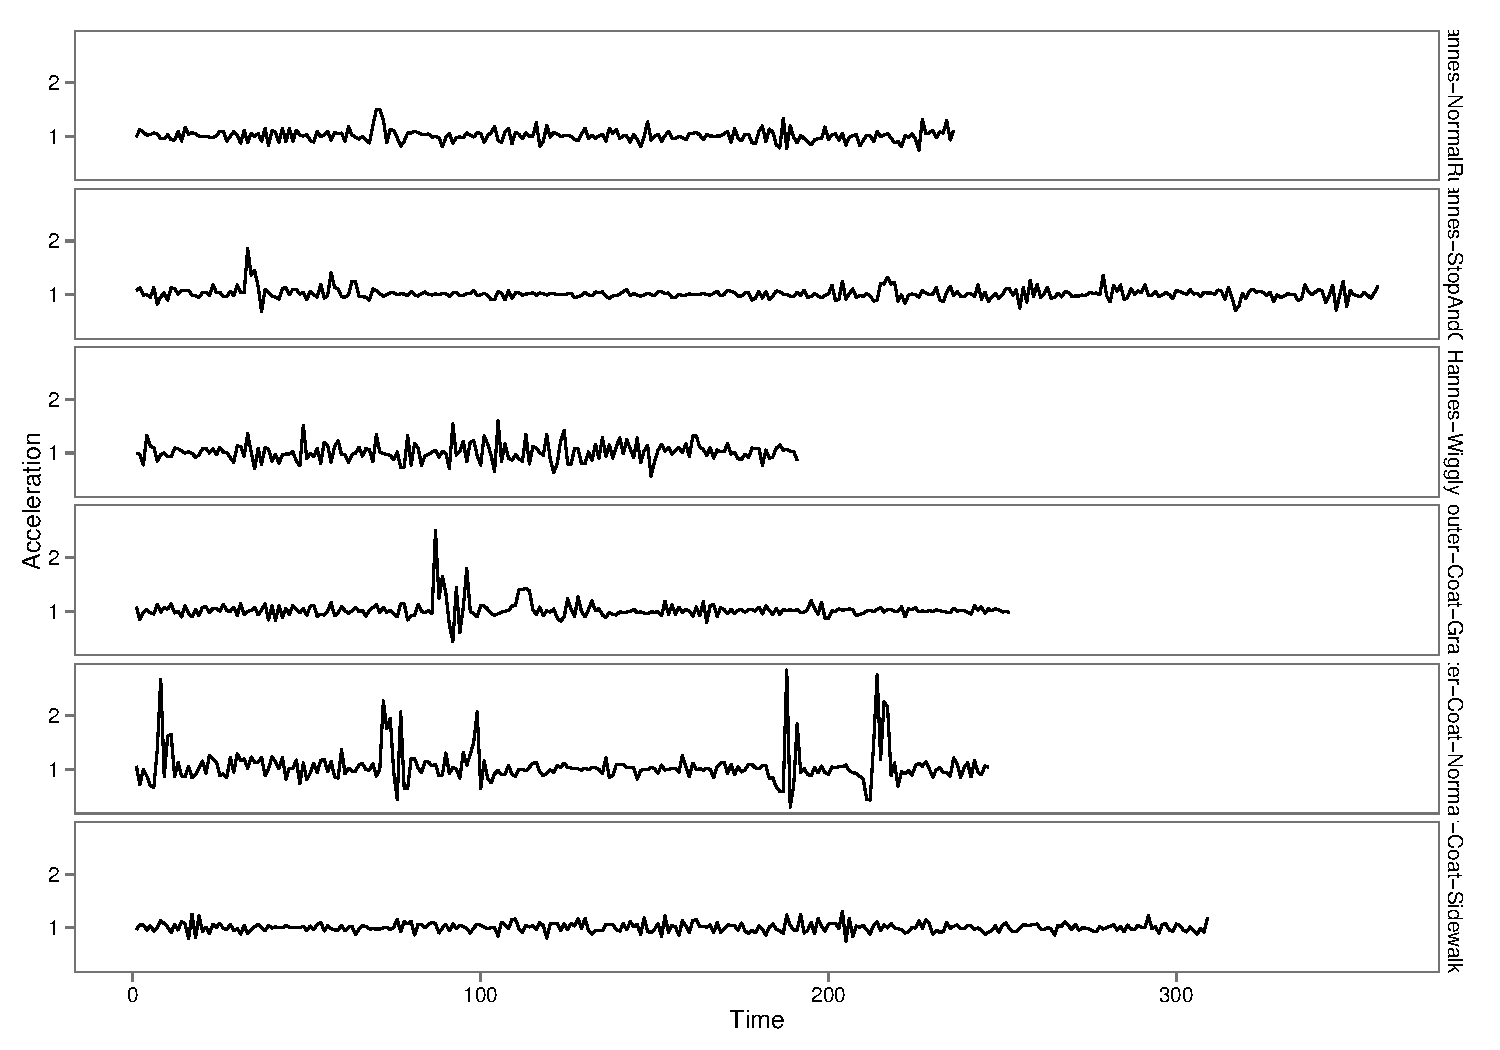
\includegraphics[width=13cm]{figures/accelerationplot-2}
\caption{Controlled experiment acceleration plot}
\label{fig:accplot2}
\end{figure}


In this experiment, we controlled for three additional factors: First, the same bike was used for all runs. Second, only two separate volunteers were used. Third, we controlled for the location of the phone on the bike, such that one rider (``Hannes'') was riding our test track with the phone taped to the bikes steering column. This setup is pictured in Figure~\ref{fig:exsetup}. The second rider (``Wouter'') would always place the phone in his coat pocked. In addition, we added different routes and riding styles. Figure~\ref{fig:accplot2} contains the acceleration vectors from this experiment. What we can see from this data is significantly more consistent and less spiky results from the runs of the first rider, which had the phone taped to the bike itself. Also, when comparing the first three plots, we can see how the riding style has a significant impact on the acceleration. At the same time, the acceleration from the second rider with the phone in the coat pocket show seemingly random fluctuations in the acceleration data. In particular, the last run, where the rider went up and down the sidewalk to induce maximum acceleration did not seem to have any effect on the acceleration, instead the inverse is apparent. From this experiment we conclude that a fixed attachment of the measuring device (such as a phone) to the bike has so far the best chances of accurate data collection. This can easily be achieved with commercially available phone holders\footnote{e.g. \url{http://www.lifeproof.com/shop/us_en/bike-mount/}}.


\subsection{Long-Run Repeated Experiment}
\begin{figure}
\centering
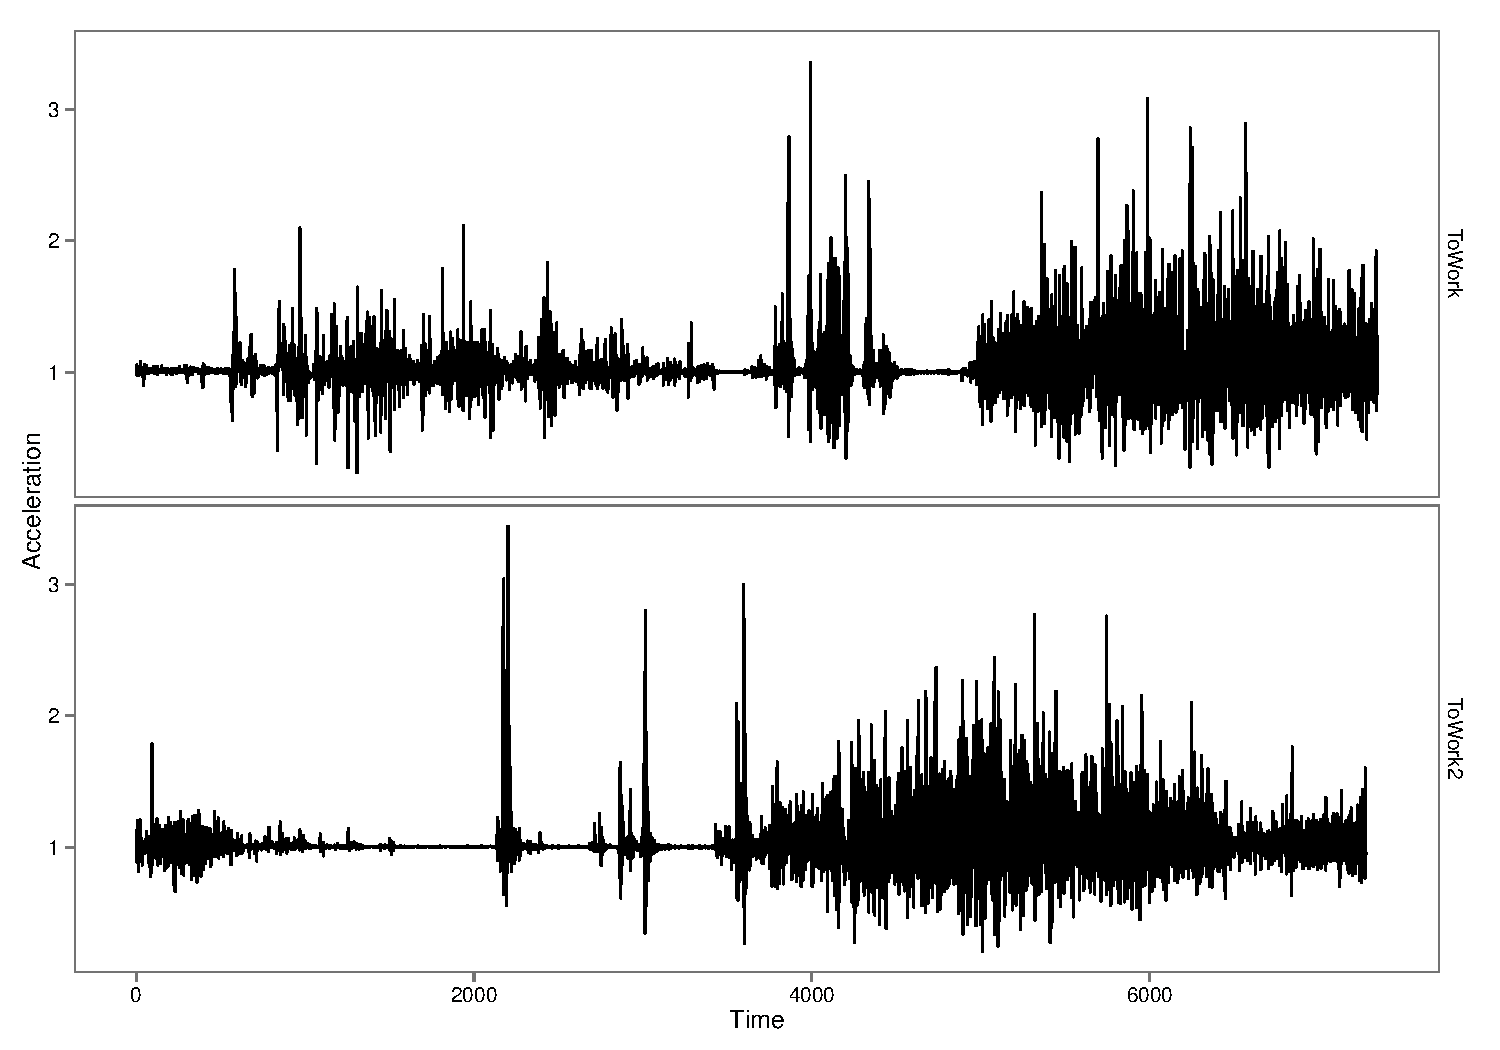
\includegraphics[width=13cm]{figures/accelerationplot-longtrack}
\caption{Final experiment acceleration plot}
\label{fig:accplotlong}
\end{figure}

To investigate the matter further, we have performed a longer experiment on a real-world bike track, which was part of the daily ride to work for one of our volunteers. The experiment track was about 2.5 kilometers long and consistet of bike roads of decreasing quality. For this experiment, the phone was also fixed to the bike as displayed in Figure~\ref{fig:exsetup}. This experiment was repeated two times. The acceleration plots are shown in Figure~\ref{fig:accplotlong}. We can see how there is a clear correlation between the two paths, albeit with a considerable time offset. Since the vertical axis of the plot is time, this can be explained through the different speeds at which the track was finished. 

\begin{figure}
\centering
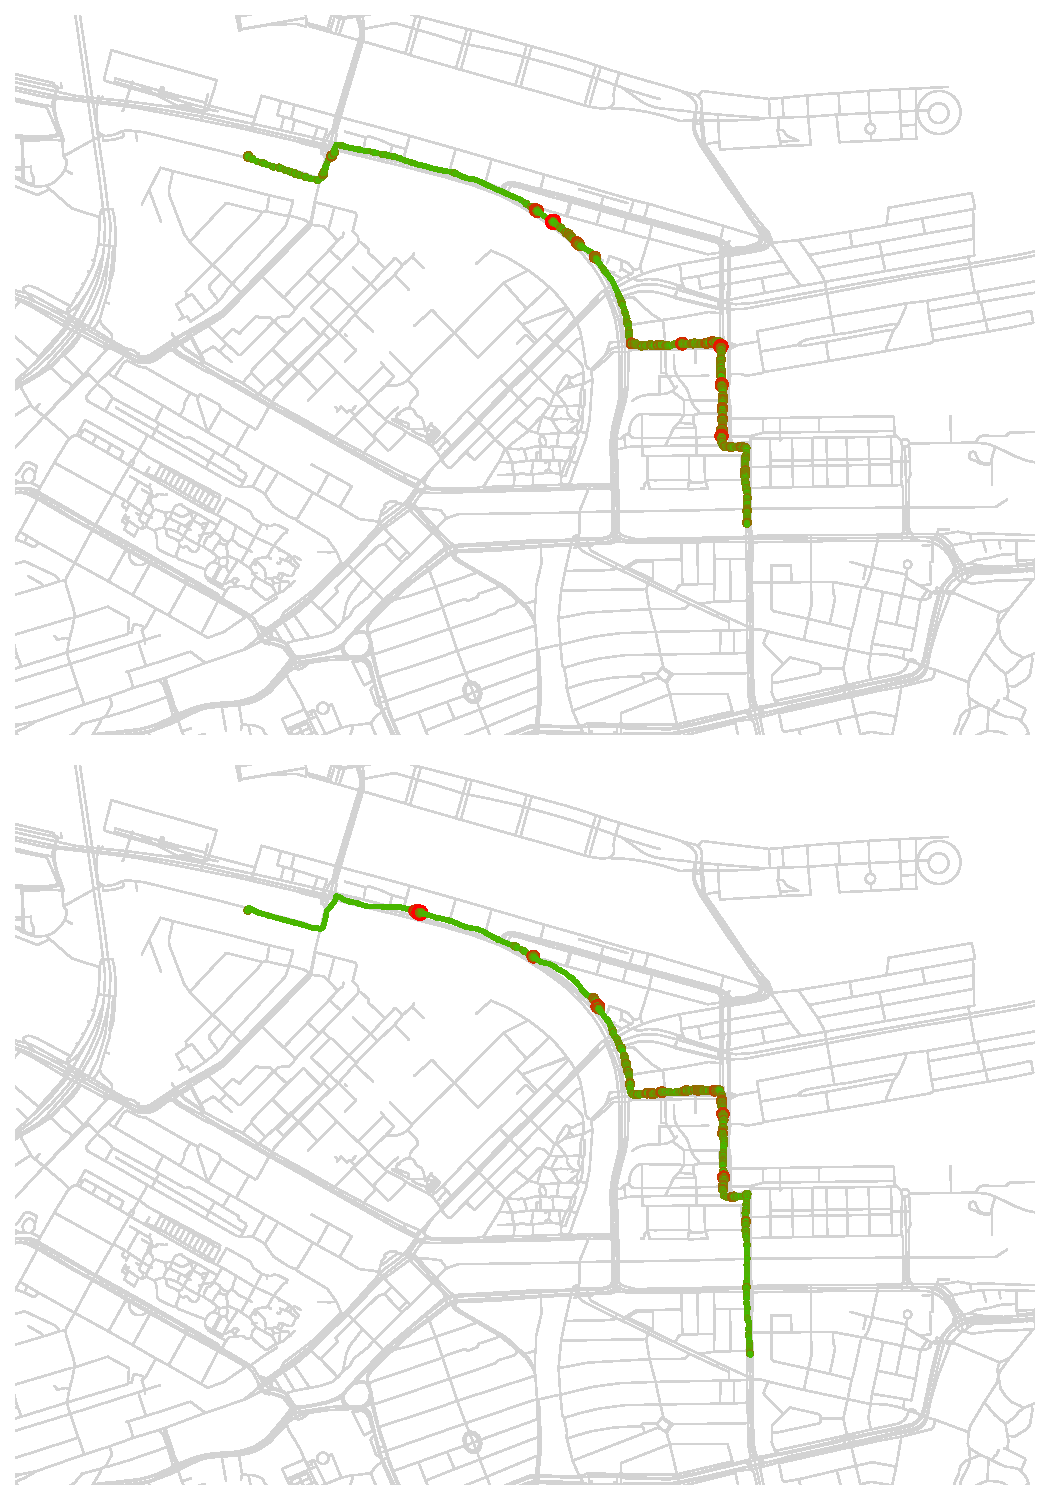
\includegraphics[width=16cm]{figures/map}
\caption{Acceleration and GPS coordinates plotted on test area map}
\label{fig:map}
\end{figure}


However, since our method of data collection also contained GPS coordinates, we were able to overlay the measured acceleration data with a map of the area. This plot is shown in Figure~\ref{fig:map}. The acceleration measurements were mapped to a color scale with gradients between green (no acceleration) and red (high acceleration). This relationship is also expressed through the different sizes of the plotted points, with a larger point representing higher acceleration as well. When comparing the two plots, we can observe that there seems to be a definitive correlation between the position of the bike and the measured acceleration. However, there are still some significant differences, for example the second track contains a large acceleration spike that the first track does not show. Of course, it is likely that the first track simply missed a pothole or a similar anomaly in the road. At the same time, there is a large spike that shows in both tracks, so we investigated further, and the bike lane is indeed very ``bumpy'' at this very position. From this experiment, we conclude that acceleration data together with position and the current time is ample information to track the bike road quality, and spurious readings can be removed given enough separate measurements.

\subsection{Data Analysis Sketch}
Given our experimental results and observations, we can describe a sketch of a data analysis system based on GPS information, time and acceleration data delivered from smart phones to a central location. 

In a first step, the acceleration data has to be normalized between particular bike, riding style and data collection device. An obvious solution would be to normalize the observed acceleration to a common scale based on the individual minimum, maximum and average values. 

Second, since individual people's tracks through a urban area are likely different, we need to split these paths up into common segments, for example based on segments of road between crossroads or housing blocks, one for each direction of travel. This allows us to compare the measurements of different participants that follow different routes. 

Third, the GPS coordinates collected might exhibit significant fluctuation, in particular when riding between buildings. However, since  timing data as well as information about the underlying road network are available, we can normalize the position data to the actual bike road. 

Last, we can the correlate the acceleration peaks between the individual road segments and positions therein. Only peaks that are consistently shown in the measured data would be eligible for future observation and reported as actual findings of bike road issues. 

It should be noted that this is a fully automated process and no human intervention is required for data collection (besides attaching a data collection device such as a phone to the bike). Similarly, the data can be analyzed without manual interaction as well. However, when considering the actual repair of the bike roads, this does not hold true any more.


\section{Related work}

The pervasiveness of smart devices has opened a number of unprecedented
opportunities for what falls under the name of \emph{crowd sensing}~\cite{gan:mob11}.
Modern smartphones have a wide plethora of sensing interfaces which make interaction with the physical
environment easy and information rich, for instance, a modern iPhone has: three-axis gyroscope, accelerometer, magnetometer, GPS, proximity
sensor, ambient light sensor, two high resolution cameras, a
microphone and high-frequency networking interfaces. These have been
exploited for a number of pattern recognition tasks, e.g.~\cite{fuj:iph10}. The specific issue of identifying the quality
of bike paths using dedicated sensors on board of bicycles has been
proposed in~\cite{eis:bik07} while possible social interactions of
bikers have been investigated
in~\cite{red:bik10}. In~\cite{eri:pot08}, the authors consider vehicle
onboard sensing to measure road quality with dedicated solutions.
Anonymous data collected by on-bike tracking devices of public bike-hire and similar schemes have been used in geospatial visualization to obtain insights in the use and effect of the scheme (e.g. \cite{krueger2014,wood2010}).

\section{Conclusions and outlook}

In this work, we have investigated the trade-offs between bike lane safety and bike 
lane information aggregation and accuracy. We have identified and prototyped an 
approach which employs off-the-shelf technology (e.g. smartphones) to report on bike lane quality,
using both online (but unconscious) and off-line support from cyclists. 
Although our initial results are promising, we identified several key
issues and their corresponding research/development areas where future work is needed:
 
\begin{itemize}\setlength{\itemsep}{-3pt}
\item Measurements alone might not be sufficient, and more complex processing steps afterwards
will require a thorough analysis on equipment investment. More complex processing 
would belong to the data analytics field (e.g. seasonal impact or other temporally correlated issues),
therefore linking this project to state-of-the-art developments in BigData.
\item Another approach to address insufficient information accuracy is to increase dramatically the number of 
measurements, which will again translate to equipment investment, as well as large-scale data analytics.
%\item KIEM project(?) / master projects
\item Computer vision state-of-the-art may be employed to further increase the accuracy of the information collected through
societal participation.
\item Social sciences could become involved in the project to support setting up a lightweight framework for dialog with stakeholders (e.g. what is available, what is possible). 
%\item Investigate privacy and security
\end{itemize}

Finally, we would recommend the setup of a pilot study, which would allow 
a deeper insight into the key issues mentioned before, as well as into those aspects 
outside the scope of this report, such as the impact on privacy and security. 

\bibliographystyle{abbrv}
\bibliography{rws}

\end{document}

